\documentclass{betterposter}

\usepackage[default]{lato}
\usepackage{inconsolata}

\usepackage{fontawesome}
\usepackage{graphicx}
\usepackage{setspace}

\definecolor{mygrey}{RGB}{63, 63, 63}

% Title font
\renewcommand{\fontsizetitle}{\fontsize{64}{80} \selectfont}

% Main column font
\renewcommand{\fontsizemain}{\fontsize{130}{200} \selectfont}

%% Setting the width of columns
% Left column
\setlength{\leftbarwidth}{0.25\paperwidth}
% Right column
\setlength{\rightbarwidth}{0.25\paperwidth}

\begin{document}
\color{mygrey}

\betterposter{%

%%% MAIN COLUMN %%%
\maincolumn{%
    \textbf{Benchmark datasets}\\
    are \textbf{not the only option}\\
    when \textbf{understanding}\\
    algorithm \textbf{performance}
}{%
    \compactqrcode{img/paper_qr.eps}{%
        \textbf{Take a picture} to\\
        download the full paper
    }%
    \hfill%
    
\includegraphics[width=.3\linewidth]{img/cu_logo}

    \vfill%
    \vspace{2em}\fontsize{40}{50}\selectfont\textbf{%
        \faGithub~\faTwitter\ \ daffidwilde
        \hfill%
        \faBook\ \ \texttt{edo.readthedocs.io}
        \hfill%
        \faNewspaperO\ \ \texttt{arxiv.org/abs/1907.13508}
    }
}

}{%

%%% LEFT COLUMN %%%
\vspace{-1ex}\title{%
    Evolutionary dataset
    \\optimisation: learning
    \\algorithm quality through
    \\evolution
}
\author{%
    \vspace{-1ex}\textbf{Henry Wilde}, Vincent Knight,
    \\Jonathan Gillard
}

\vspace{-1em}\section{Motivating paradigm}
\vspace{-1.5em}\begin{center}
    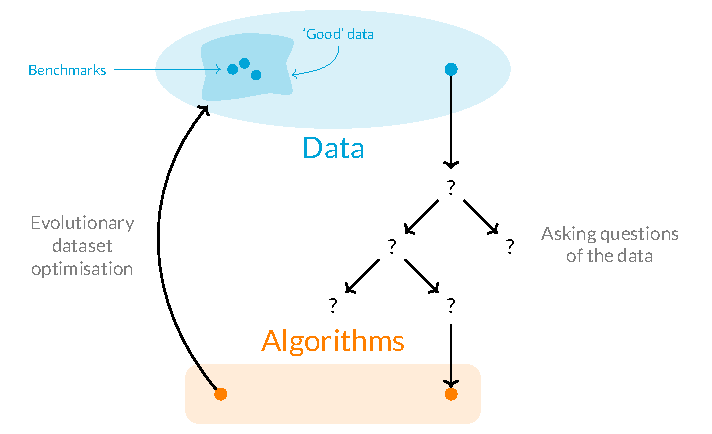
\includegraphics[width=.9\linewidth]{tex/paradigm.pdf}
\end{center}

\textcolor{mygrey}{%
    \textit{Left:} the proposed concept to understand algorithm performance by
    exploration of `good' (or bad) datasets. \textit{Right:} the established
    approach to algorithm selection by metric comparison.
}

\vspace{-.5em}\section{Using an evolutionary\\algorithm}

\vspace{-1em}\begin{minipage}{.04\linewidth}
    \
\end{minipage}
\begin{minipage}{.9\linewidth}
    \begin{itemize}
        \renewcommand\labelitemi{\faThumbsOUp~}
        \item Effective in complex domains
        \item Meaningful and adjustable design
        \item Transparent and rich solutions
    \end{itemize}

    \vspace{1ex}\begin{itemize}
        \renewcommand\labelitemi{\faThumbsODown~}
        \item Potential suboptimal termination
        \item Finds the `easy' way out
        \item Requires careful consideration of fitness
    \end{itemize}
\end{minipage}


\section{A case study in clustering}

\vspace{-1.5em}\begin{center}
    \begin{minipage}{.8\linewidth}
        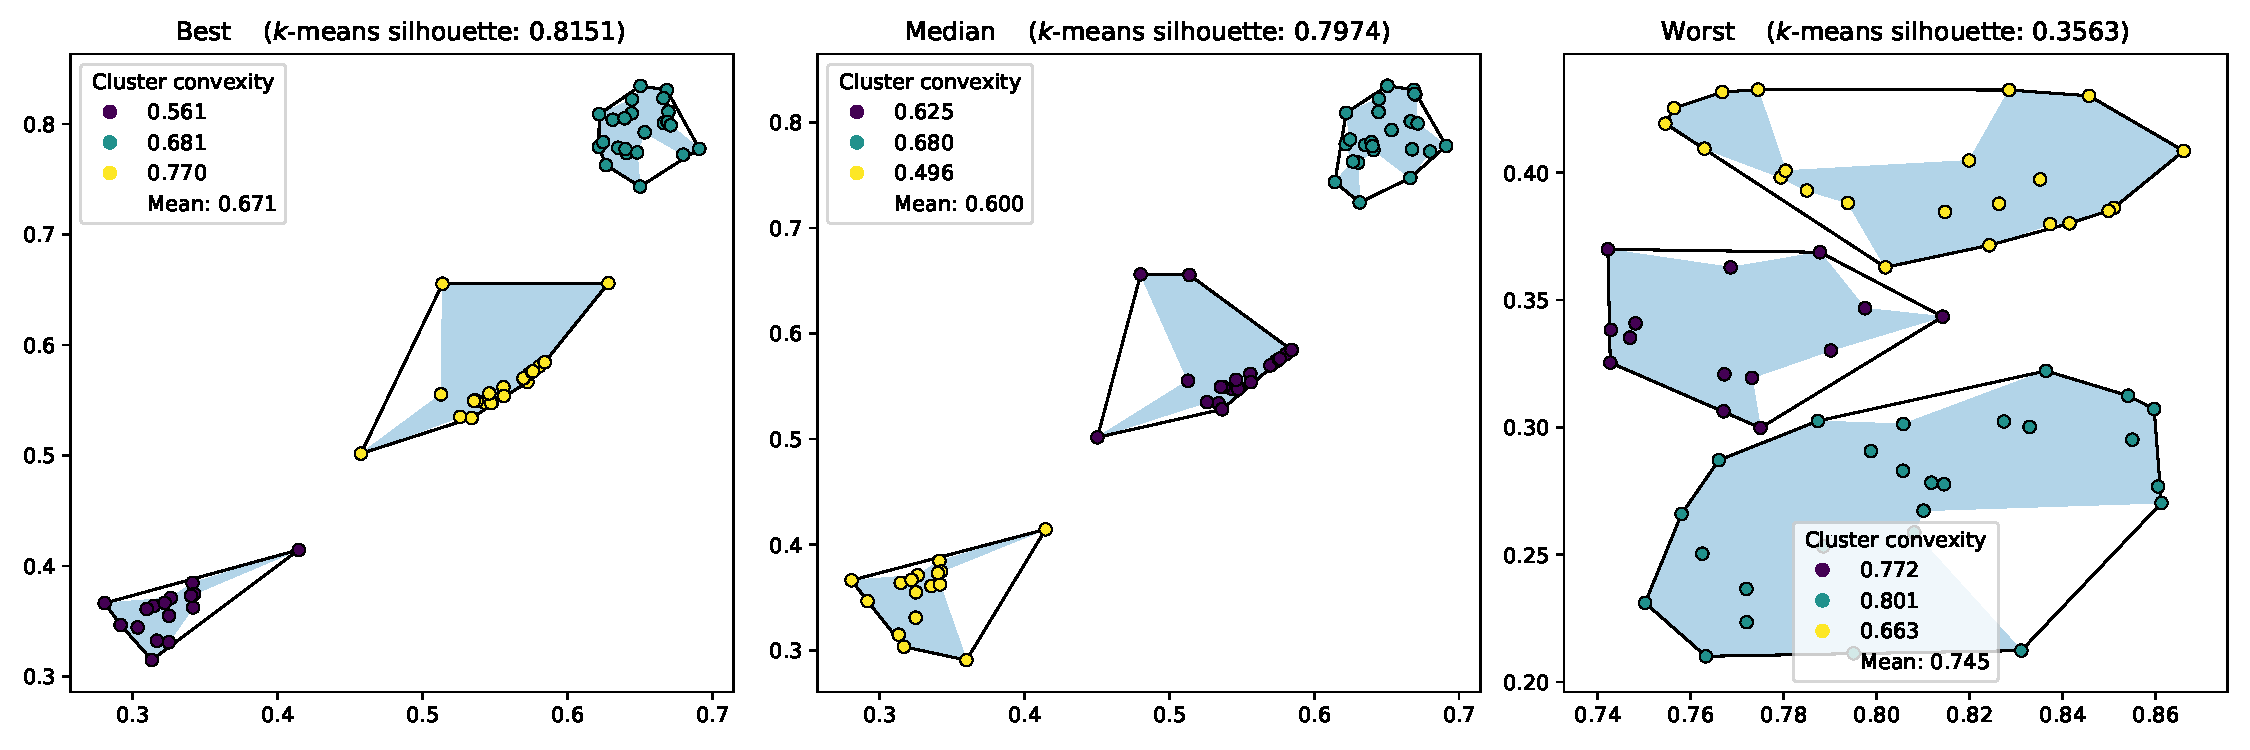
\includegraphics[width=\linewidth]{img/kmeans.pdf}\vspace{1ex}

        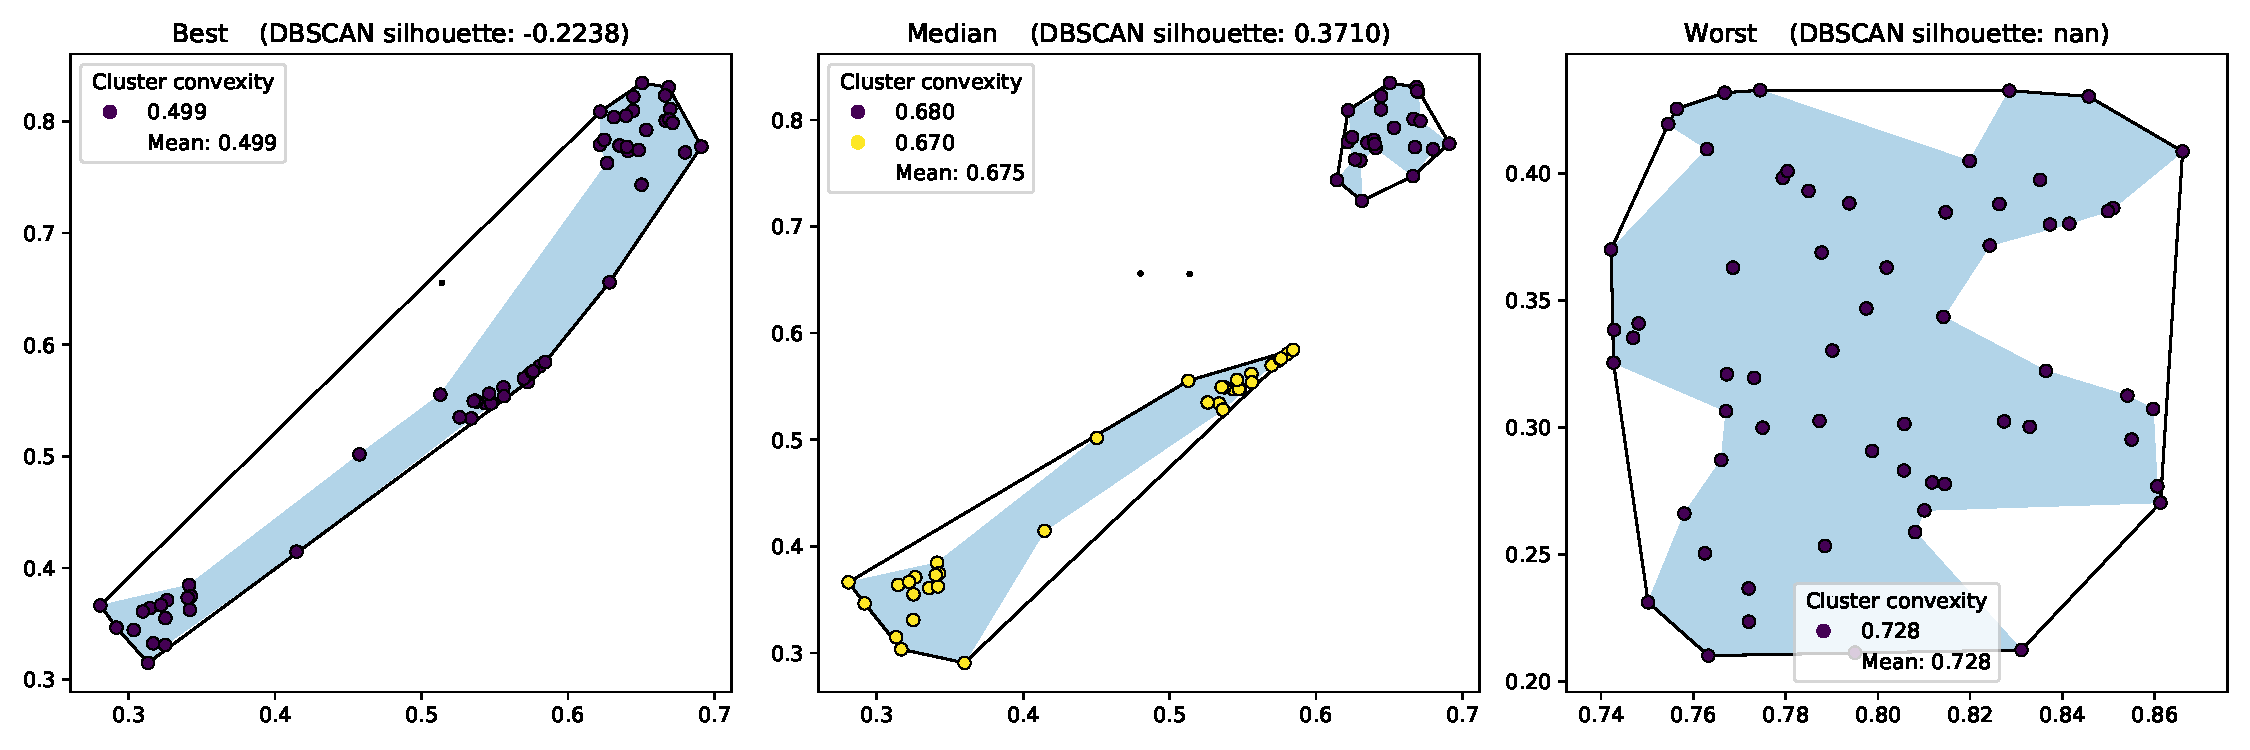
\includegraphics[width=\linewidth]{img/dbscan.pdf}
    \end{minipage}
\end{center}

\textcolor{mygrey}{%
    Best and worst datasets from attempt to maximise the silhouette of
    \(k\)-means (\textit{top}) whilst minimising that of DBSCAN
    (\textit{bottom}).
}

}{%

%%% RIGHT COLUMN %%%

\vspace{-3em}\section{Inner mechanisms}
\fontsize{40}{50}\selectfont
Individual dataset representation

\vspace{.75ex}\begin{center}
    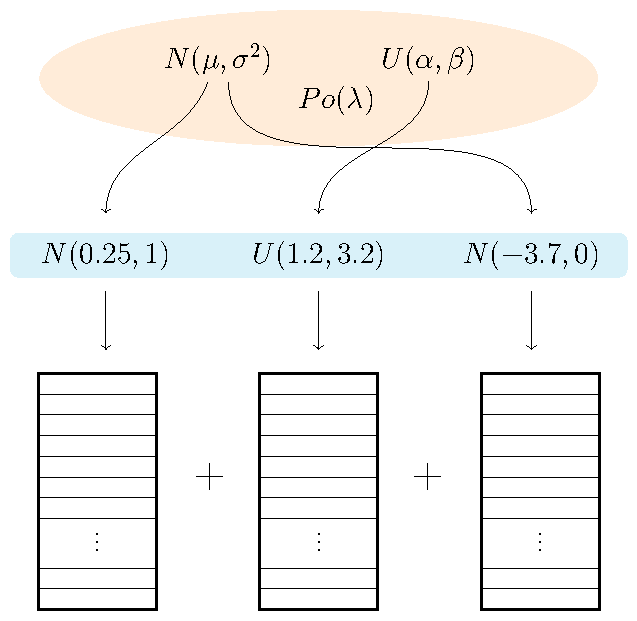
\includegraphics[width=.65\linewidth]{tex/individual.pdf}
\end{center}

Modified truncation selection

\vspace{.75ex}\begin{center}
    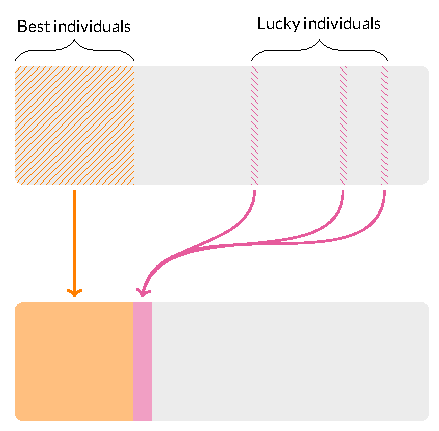
\includegraphics[width=.65\linewidth]{tex/selection.pdf}
\end{center}

Uniform-sampling crossover

\vspace{.75ex}\begin{center}
    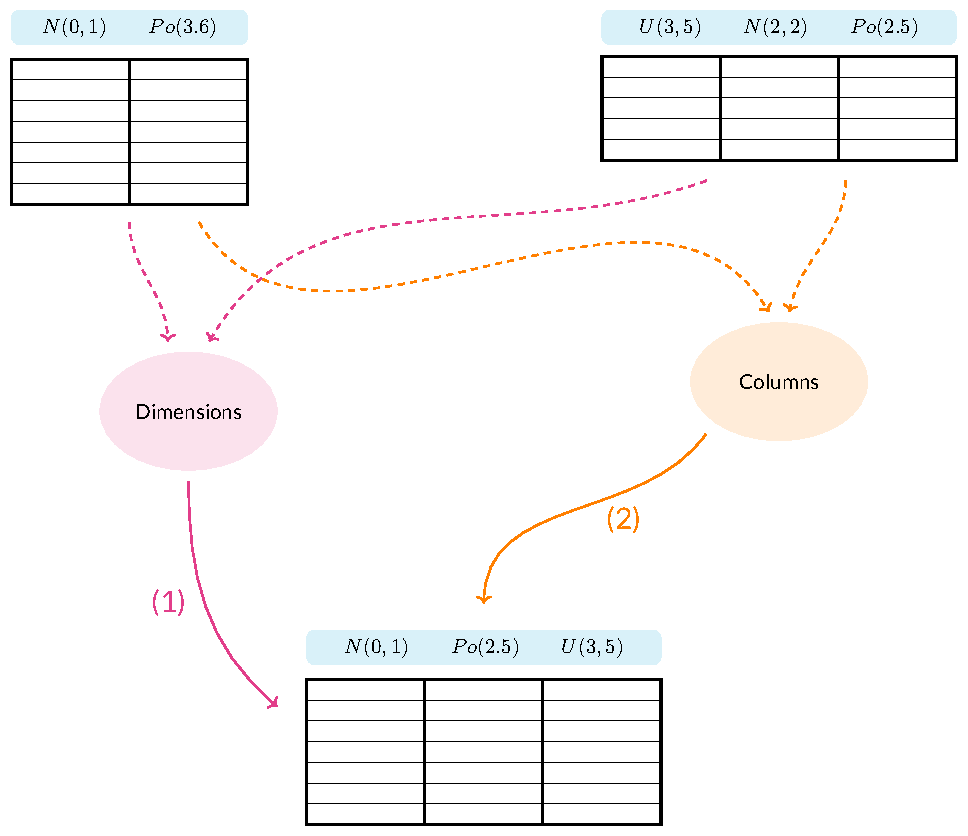
\includegraphics[width=.8\linewidth]{tex/crossover.pdf}
\end{center}

Mutation process adapted for datasets

\vspace{.75ex}\begin{center}
    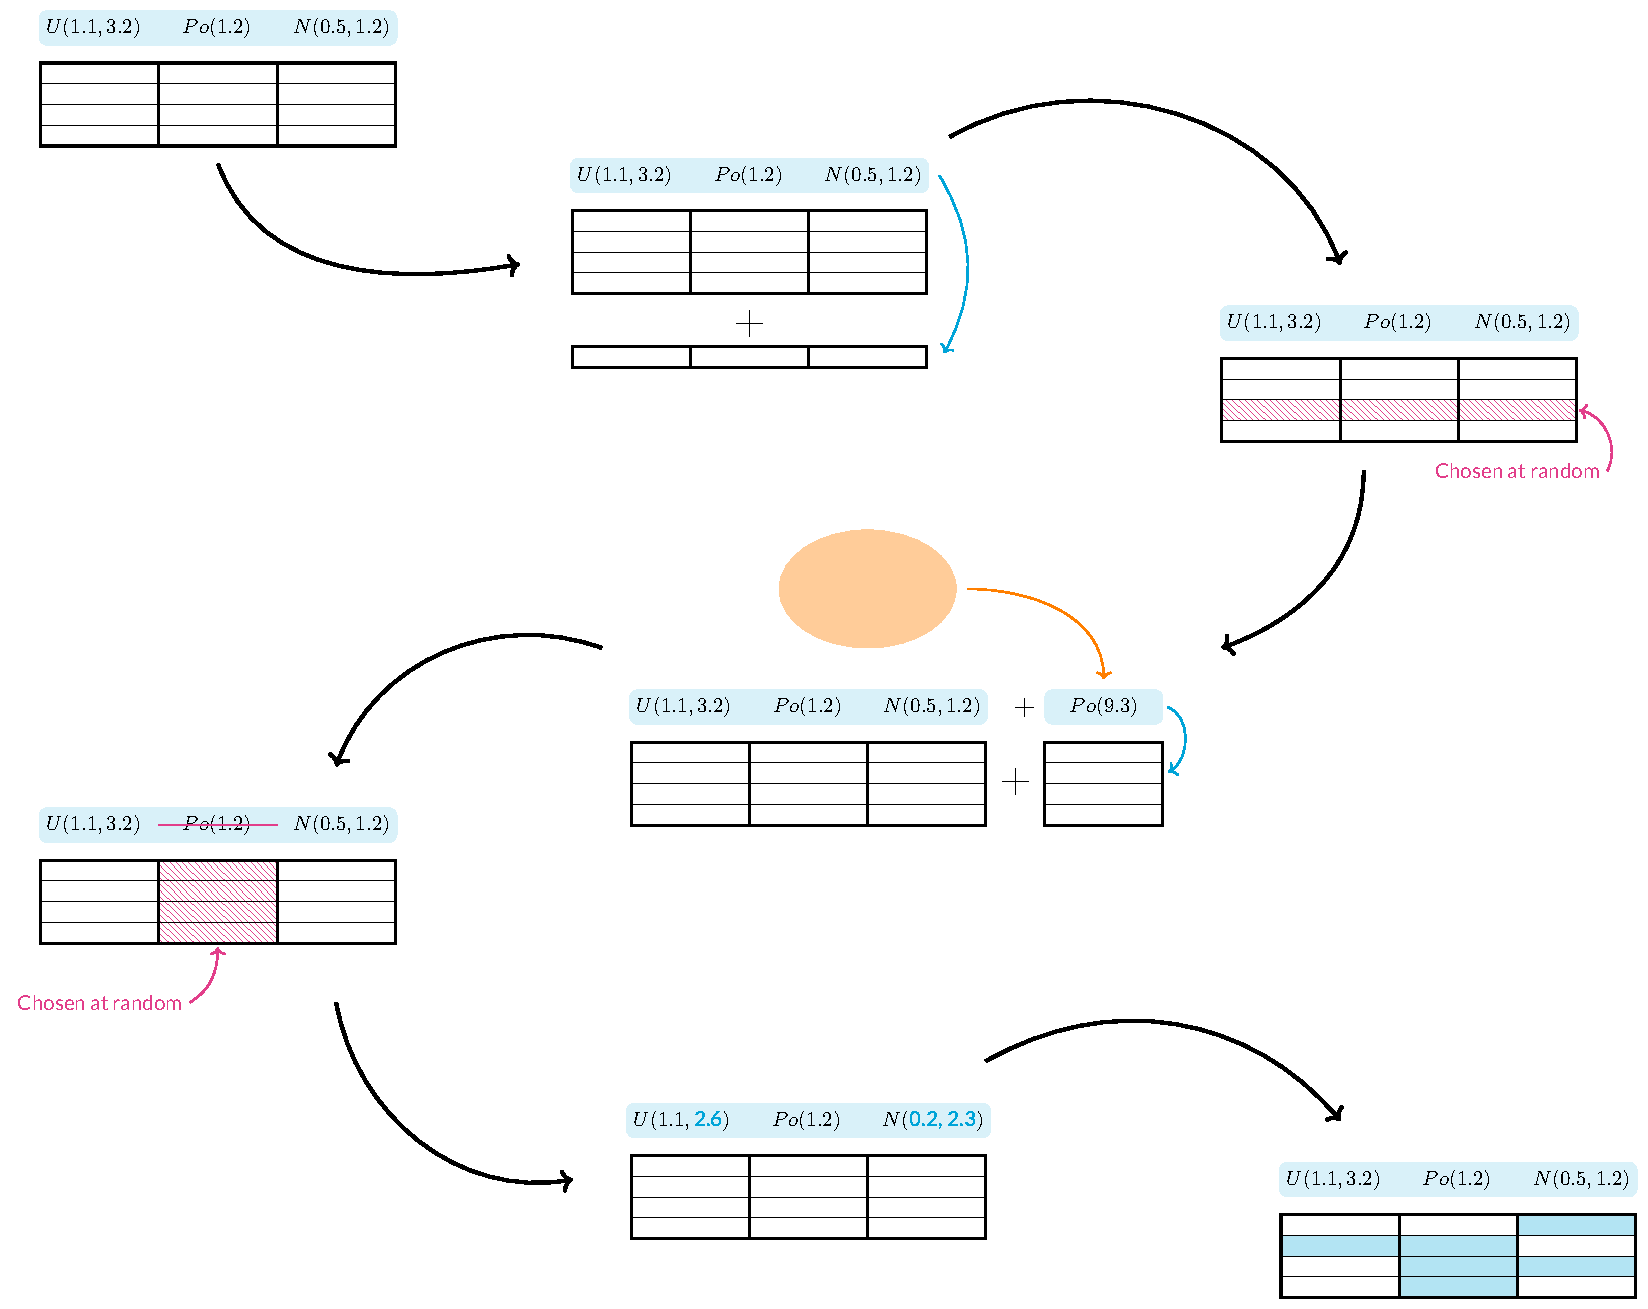
\includegraphics[width=.9\linewidth]{tex/mutation.pdf}
\end{center}
}

\end{document}
